\chapter{ПОСТРОЕНИЕ ГЕНЕРАТОРА ПОСЛЕДОВАТЕЛЬНОСТИ}
\label{cha:lab2}
	
\section {Постановка задачи}
Требуется описать конечный автомат, представляющий собой генератор
фиксированной последовательности логических сигналов, в виде синтезируемой модели
на языке Verilog HDL.
Автомат должен иметь интерфейс, представленный на Рисунке~\ref{fig:fsmexample}.

% TODO: \usepackage{graphicx} required
\begin{figure}[h!]
	\centering
	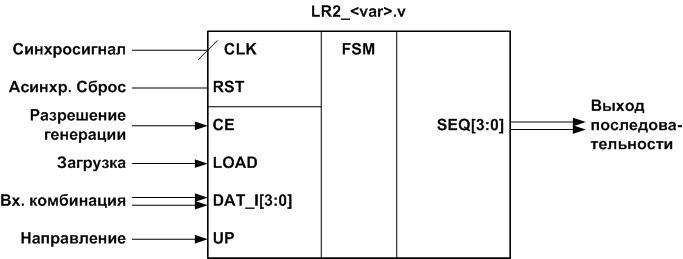
\includegraphics[width=0.6\linewidth]{course-plis/images/lab2/fsm_example}
	\caption{Интерфейс цифрового автомата}
	\label{fig:fsmexample}
\end{figure}


Автомат является синхронным цифровым узлом, срабатывающим по восходящим
фронтам синхросигнала \textit{CLK}. Исключение составляет асинхронный вход сброса \textit{RST},
принудительно устанавливающий регистр автомата в исходное состояние (определяется
вариантом).
Автомат должен реагировать на входные воздействия согласно Таблице~\ref{tab:fsm state}.


\begin{table}[h!]
	\centering
		\caption{Таблица функционирования автомата}
		\small
	\begin{tabular}{|c|c|c|c|c|c|}
		\hline
		\textbf{RST}  & \textbf{CLK}  & \textbf{LOAD}  & \textbf{CE}  & \textbf{UP}  & \textbf{Действие} \\ \hline \hline
		1 & X  & X  & X  & X  & Асинхронный сброс SEQ <= Func(4'h0) \\ \hline
		0 & posedge & 1 & X  & X  & Загрузка SEQ <= Func(DAT\_I) \\ \hline
		0 & posedge & 0 & 1 & 0 & Обратная генерация SEQ <= Func(i-1) \\ \hline
		0 & posedge & 0 & 1 & 1 & Прямая генерация SEQ <= Func(i+1) \\ \hline
		0 & posedge & 0 &  & X  & Хранение SEQ <= SEQ \\ \hline
	\end{tabular}
	\label{tab:fsm state}
\end{table}


Последовательность генерируемых сигналов определяется функцией~\\\textit{Func(i)}, где \textit{i} --- четырехразрядный двоичный индекс, представляющий собой номер элемента
последовательности. 
Инкремент индекса соответствует прямой генерации последовательности.
Декремент индекса соответствует обратной генерации последовательности.

Последовательность для каждого варианта выполнения работы определяется из
таблицы вариантов следующим образом: индекс \textit{i} задан входными комбинациями от \textit{F} до
0 в верхней строке таблицы, а выходные комбинации \textit{Func(i)}, формируемые на выходах
\textit{SEQ[3:0]}, заданы строкой таблицы, соответствующей выбранному варианту.
Допускается использовать различные варианты кодировки состояний автомата.
Автомат может иметь организацию согласно абстрактным моделям Мили или Мура.

\section {Реализация конечного автомата}
Требуется описать конечный автомат, представляющий собой генератор
фиксированной последовательности логических сигналов, в виде синтезируемой модели
на языке Verilog HDL согласно данной таблице истинности и вектор-функции (см. Таблицу~\ref{tab:func-vector}).

\begin{table}[h!]
	\centering
	\caption{Вектор-функция}
		\begin{tabular}{|c|c|c|c|c|c|c|c|c|c|c|c|c|c|c|c|}
			\hline
			F & E & D & C & B & A & 9 & 8 & 7 & 6 & 5 & 4 & 3 & 2 & 1 & 0 \\ \hline\hline
			0 & 4 & 4 & 8 & 3 & 0 & 7 & 2 & 2 & D & 7 & C & 5 & 2 & A & C \\ \hline
		\end{tabular}
		\label{tab:func-vector}
\end{table}

\section{Структурная схема автомата}
Построим структурную схему цифрового устройства. Используем делитель частоты для снижения частоты тактового генератора, фильтр дребезга для использования кнопок в качестве устройств ввода (см. Рисунок~\ref{fig:fsm-struct}).
% TODO: \usepackage{graphicx} required
\begin{figure}[htpb]
	\centering
	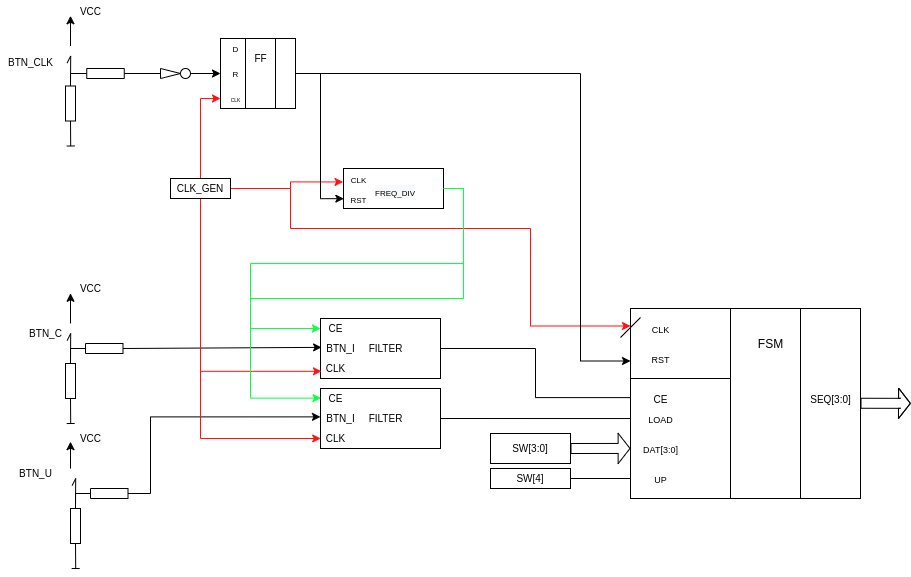
\includegraphics[width=\linewidth]{course-plis/images/lab2/fsm-struct}
	\caption{Структурная схема  устройства}
	\label{fig:fsm-struct}
\end{figure}


\section{Кодировка состояний автомата в двоичной и шестнадцатиричной системах}
Опишем модуль behaviour.v, указав в нем состояния автомата, приведенные в шестнадцатеричной системе.
Исходный код данного модуля приведен в Приложении~\ref{cha:appendix1} на Листинге~\ref{lst:1beh}.


%\newpage
\section{Граф состояний}
Опишем граф перехода цифрового автомата согласно указанным режимам работы (переход в следующее или предыдущее состояние, загрузка состояния, хранение, сброс) (см. Рисунок~\ref{fig:graph}).
% TODO: \usepackage{graphicx} required
\begin{figure}[h!]
	\centering
	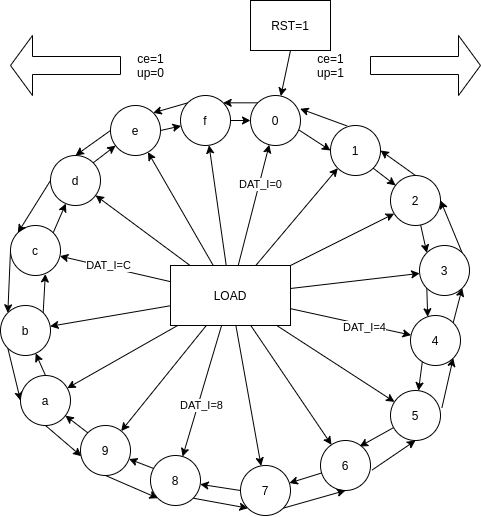
\includegraphics[width=0.4\linewidth]{course-plis/images/lab2/graph}
	\caption{Граф переходов}
	\label{fig:graph}
\end{figure}

\newpage
\section{Создание проекта САПР Xilinx ISE}

\paragraph{Автомат генератор последовательности.}
Реализуем на языке Verilog модуль, описывающий цифровой автомат. 
Исходный код данного модуля приведен в Приложении~\ref{cha:appendix1} на Листинге~\ref{lst:2fsm}.
\paragraph{Делитель частоты.}
Реализуем на языке Verilog модуль, описывающий делитель частоты.
Исходный код данного модуля приведен в Приложении~\ref{cha:appendix1} на Листинге~\ref{lst:2freq-div}.

\paragraph{Фильтр дребезга кнопок.}
Реализуем на языке Verilog модуль, описывающий фильтр дребезга.
Исходный код данного модуля приведен в Приложении~\ref{cha:appendix1} на Листинге~\ref{lst:2filter}.

\paragraph{Модуль верхнего уровня.}
Реализуем на языке Verilog модуль верхнего уровня.
Исходный код данного модуля приведен в Приложении~\ref{cha:appendix1} на Листинге~\ref{lst:2top}.


\paragraph{Тестовое окружение.}
Реализуем на языке Verilog модуль, описывающий тестовое окружение, описывающее входные воздействия для данной модели.
Исходный код данного модуля приведен в Приложении~\ref{cha:appendix1} на Листинге~\ref{lst:2fsm-test}.


\section{Тестирование и отладка средствами симулятора iSim}
После компоновки проекта, подключения модуля верхнего уровня, проведем верификацию спроектированных моделей с помощью симулятора iSim из состава САПР Xilinx ISE Design Suite. Результаты тестирования можно видеть в Приложении~\ref{cha:appendix2} на Рисунках~\ref{fig:2isim1}.~\ref{fig:2isim2}.



\section{Вывод}
  В данном разделе нами были получены общие навыки работы с программным обеспечением Xilinx ISE Design Suite, изучены основы языка Verilog.

С помощью полученных знаний был спроектирован конечный автомат, представляющий собой генератор
фиксированной последовательности логических сигналов, в виде синтезируемой модели.

